\begin{frame}
    \titlepage{}
\end{frame}

\begin{frame}{Этапы парсинга}
    \begin{enumerate}
        \item Выделение лексем
        \item Преобразование потока лексем в нативные структуры
    \end{enumerate}
\end{frame}

\begin{frame}{Требования к парсеру}
    \begin{enumerate}
        \item Гарантии
        \item Эргономика
        \item Производительность
    \end{enumerate}
\end{frame}

\begin{frame}{Про кого поговорим}
    \begin{itemize}
        \item \href{https://docs.rs/nom/latest/nom/}{nom}
        \item \href{https://docs.rs/combine/latest/combine/}{combine}
        \item \href{https://docs.rs/chumsky/latest/chumsky/}{chumsky}
        \item \href{https://docs.rs/pest/latest/pest/}{pest}
        \item \href{https://github.com/lalrpop/lalrpop}{lalrpop}
    \end{itemize}
\end{frame}

\begin{frame}[fragile]{Почему не NOM}
    \begin{minted}[style = manni, fontsize=\footnotesize]{rust}
fn bool(source: &str) -> IResult<&str, Query> {
    alt((value(true, tag("true")), value(false, tag("false")))).map(Query::Value)
        .parse(source)
}

fn not(source: &str) -> IResult<&str, Query> {
    tag("-").and_then(query).map(|q| Query::Not(q.into())).parse(source)
}

pub fn query(source: &str) -> IResult<&str, Query> {
    let or = |source| many2(query, tag("|"), source);
    let and = |source| many2(query, tag("|"), source); // <-- bug here
    let bracketed = tuple((tag("("), query, tag(")"))).map(|(_, q, _)| q);
    alt((bool, not, or.map(Query::Or), and.map(Query::And), bracketed))(source)
}
    \end{minted}
\end{frame}

\begin{frame}[fragile]{Почему LALRPOP}
    \begin{minted}[style = manni, fontsize=\footnotesize]{rust}
Boolean: bool = { "true" => true, "false" => false };
Value: Query = Boolean => Query::Value(<>);

NotInner = { Value, "(" <Or> ")", "(" <And> ")" };
Not: Query = "-" <NotInner> => Query::Not(<>.into());

AndOrLeaf = { Value, "(" <Or> ")", "(" <And> ")", Not}
And: Query = Many2<AndOrLeaf, "|"> => Query::And(<>); // <-- bug here
Or: Query = Many2<AndOrLeaf, "|"> => Query::Or(<>);

pub Query: Query = {
    Value, And, Or, Not,
}
    \end{minted}
\end{frame}

\begin{frame}[fragile]{Почему не chumsky}
    \begin{minted}[style = manni, fontsize=\footnotesize]{rust}
fn float() -> impl Parser<char, f64, Error = Simple<char>> {
    let frac = just('.').chain(digits(10));
    let exp = just('e').or(just('E'))
        .chain(just('+').or(just('-')).or_not())
        .chain::<char, _, _>(digits(10));

    just('-')
        .or_not()
        .chain::<char, _, _>(int(10))
        .chain::<char, _, _>(frac.or_not().flatten())
        .chain::<char, _, _>(exp.or_not().flatten())
        .collect::<String>().from_str().unwrapped()
        .labelled("float")
}
    \end{minted}
\end{frame}

\begin{frame}{Обзор инструментов}
    \large\begin{table}[]
        \begin{tabular} { |l|l|l|l|l|l|l| }
            \hline
                               & NOM & Combine & Chumsky & pest & peg & LALRPOP \\ \hline
            Гарантии           & 0   & 0       & 0       & 0    & 0   & 5       \\ \hline
            Эргономика         & 1   & 4       & 4       & 3    & 3   & 4       \\ \hline
            Производительность & 5   & 5       & 2       & 2    & 2   & 4       \\ \hline
        \end{tabular}
    \end{table}
\end{frame}

\begin{frame}
    \begin{itemize}
      \item Базовые математические операции: сложение, вычитание, деление, умножение.
      \item Функции:
      \begin{itemize}
        \item Встроенные: sin, cos, pi.
        \item Определяемые пользоваетелем.
      \end{itemize}
    \end{itemize}
\end{frame}

\begin{frame}[fragile]{Eva}
    \begin{minted}[style = manni, fontsize=\large]{rust}
fn constant() = 42.0;

fn double(fst, snd) = fst * snd;

fn triple(fst, snd, thrd) = double(fst, snd) * thrd;

cos(triple(2.0, constant() * pi(), 8.0 / 2.0))
    \end{minted}
\end{frame}

\begin{frame}[fragile]{Expression}
    \begin{minted}[style = manni, fontsize=\footnotesize]{rust}
pub enum Expression<V> {
    Value(V),

    Op {
        left: Box<Self>,
        op: Operation,
        right: Box<Self>,
    },

    FnCall {
        function: Function,
        arguments: Vec<Self>,
    },
}
    \end{minted}
\end{frame}

\begin{frame}[fragile]{Operation}
    \begin{minted}[style = manni, fontsize=\large]{rust}
pub enum Operation {
    Sum,
    Mul,
    Div,
    Sub,
}
    \end{minted}
\end{frame}

\begin{frame}[fragile]{FunctionValue}
    \begin{minted}[style = manni, fontsize=\Large]{rust}
pub enum FunctionValue {
    Float(f64),
    Variable(String),
}
    \end{minted}
\end{frame}

\begin{frame}[fragile]{UserDefinedFunction}
    \begin{minted}[style = manni, fontsize=\large]{rust}
pub struct UserDefinedFunction {
    pub(crate) name: String,
    pub(crate) args: Vec<String>,
    pub(crate) expression: Expression<FunctionValue>,
}
    \end{minted}
\end{frame}

\begin{frame}[fragile]{LALRPOP intro}
    \begin{minted}[style = manni, fontsize=\normalsize]{rust}
use crate::Name;

grammar;

pub(crate) Expression: Name = {
    "(" <r"\p{alpha}+"> ")" => Name::new(<>),

    "[" <name:r"\p{alpha}+"> "]" =>? {
        let result = Name::try_new(name)?,
        Ok(result)
    },
}
    \end{minted}
\end{frame}

\begin{frame}[fragile]
    \begin{minted}[style = manni, fontsize=\footnotesize]{rust}
use std::str::FromStr;
use crate::prelude::*;

grammar(context: &mut Context);
extern {
    type Error = Error;
}

// (foo, bar, baz) | (2.1, 3.0) | (1.2, bar, fuz,) | ()
Args<T>: Vec<T> = {
    "(" <mut args: (<T> ",")*> <last: T?> ")" => {
        if let Some(last) = last {
            args.push(last);
        }
        args
    }
}
    \end{minted}
\end{frame}

\begin{frame}[fragile]
    \begin{minted}[style = manni, fontsize=\footnotesize]{rust}
ExprOp: Operation = {
    "+" => Operation::Sum,
    "-" => Operation::Sub,
}

FactorOp: Operation = {
    "*" => Operation::Mul,
    "/" => Operation::Div,
}

Float: f64 = r"-?\d+(\.\d*)?" => f64::from_str(<>).unwrap();
Name: String = r"\p{alpha}+" => <>.into();

FunctionValue: FunctionValue = {
    Float => <>.into(),
    Name => <>.into(),
}
    \end{minted}
\end{frame}

\begin{frame}[fragile]
    \begin{minted}[style = manni, fontsize=\footnotesize]{rust}
Term<Value>: Expression<Value> = {
    Value => Expression::Value(<>),
    "(" <Expression<Value>> ")",
    <name:Name> <arguments:Args<Expression<Value>>> =>? {
        let call = Expression::function_call(context, name, arguments)?;
        Ok(call)
    }
}

Tier<Value, Operation, Right>: Expression<Value> = {
    Tier<Value, Operation, Right> Operation Right => Expression::op(<>),
    Right,
}

Factor<Value> = Tier<Value, FactorOp, Term<Value>>;
Expression<Value> = Tier<Value, ExprOp, Factor<Value>>;
    \end{minted}
\end{frame}

\begin{frame}[fragile]
    \begin{minted}[style = manni, fontsize=\footnotesize]{rust}
Function: () = {
    "fn" <n:Name>
         <args: Args<Name>>
        "="
        <expr:Expression<FunctionValue>>
        ";"
    =>? {
        let function = UserDefinedFunction::new(n.clone(), args, expr)?;
        context.add_function(n, function)?;
        Ok(())
    }
}

pub TopLevelExpression: Expression<f64> = {
    Function* <r:Expression<Float>> => r,
}
    \end{minted}
\end{frame}

\begin{frame}
  \textbf{Генерация тестовых данных}
\end{frame}

\begin{frame}[fragile]
    \begin{minted}[style = manni, fontsize=\footnotesize]{rust}
pub fn value() -> impl Strategy<Value = f64> + Clone {
    any::<f64>().prop_filter("Values must be comparable.", |x| x.is_normal())
}

pub fn function_value(variables: Vec<String>)
-> impl Strategy<Value = FunctionValue> + Clone {
    prop_oneof![
        5 => value().prop_map(FunctionValue::Float),
        1 => select(variables).prop_map(FunctionValue::Variable)
    ]
}
    \end{minted}
\end{frame}

\begin{frame}[fragile]
    \begin{minted}[style = manni, fontsize=\footnotesize]{rust}
fn term<S: Strategy<Value = V> + Clone + 'static, V: Clone + Debug + 'static>(
    value_strategy: S,
    user_defined_functions: Vec<Arc<UserDefinedFunction>>,
) -> impl Strategy<Value = Expression<V>> {
    prop_oneof![
        10 => value_strategy.clone().prop_map(Expression::Value),
        1 => function_call(value_strategy, user_defined_functions),
    ]
}
    \end{minted}
\end{frame}

\begin{frame}[fragile]
    \begin{minted}[style = manni, fontsize=\footnotesize]{rust}
fn user_defined_function(
    functions: Vec<Arc<UserDefinedFunction>>,
) -> impl Strategy<Value = UserDefinedFunction> {
    (
        r"\p{alpha}{8,16}",
        proptest::collection::hash_set(r"\p{alpha}{3,7}", 2..5),
    )
        .prop_flat_map(move |(name, args)| {
            let args = args.into_iter().collect::<Vec<_>>();
            expression(function_value(args.clone()), functions.clone()).prop_map(
                move |expression| UserDefinedFunction {
                    name: name.clone(),
                    args: args.clone(),
                    expression,
                },
            )
        })
}
    \end{minted}
\end{frame}

\begin{frame}[fragile]
    \begin{minted}[style = manni, fontsize=\scriptsize]{rust}
fn function_call<S: Strategy<Value = V> + Clone + 'static, V: Clone + Debug + 'static>(
    value_strategy: S, user_defined_functions: Vec<Arc<UserDefinedFunction>>,
) -> impl Strategy<Value = Expression<V>> {
    if user_defined_functions.is_empty() {
        any::<BuiltinFunction>().prop_map(Into::<Function>::into).boxed()
    } else { prop_oneof![
            1 => select(user_defined_functions.clone()).prop_map(Function::UserDefined),
            10 => any::<BuiltinFunction>().prop_map(Into::<Function>::into),
    ].boxed() }
    .prop_flat_map(move |function| { prop::collection::vec(
            expression(value_strategy.clone(), user_defined_functions.clone()),
            function.arguments_count(),
        )
        .prop_map(move |arguments| Expression::FnCall {
            function: function.clone(),
            arguments,
    })})
}
    \end{minted}
\end{frame}

\begin{frame}[fragile]
    \begin{minted}[style = manni, fontsize=\footnotesize]{rust}
fn factor<S: Strategy<Value = V> + Clone + 'static, V: Clone + Debug + 'static>(
    strategy: S,
    user_defined_functions: Vec<Arc<UserDefinedFunction>>,
) -> impl Strategy<Value = Expression<V>> {
    term(strategy.clone(), user_defined_functions.clone())
        .prop_recursive(4, 16, 4, move |inner| {
            (
                inner,
                prop_oneof![Just(Mul), Just(Div)],
                term(strategy.clone(), user_defined_functions.clone()),
            )
                .prop_map(|(left, op, right)| Expression::op(left, op, right))
        })
}
    \end{minted}
\end{frame}

\begin{frame}[fragile]
    \begin{minted}[style = manni, fontsize=\scriptsize]{rust}
fn expression<S: Strategy<Value = V> + Clone + 'static, V: Clone + Debug + 'static>(
    value_strategy: S,
    user_defined_functions: Vec<Arc<UserDefinedFunction>>,
) -> impl Strategy<Value = Expression<V>> {
    factor(value_strategy.clone(), user_defined_functions.clone())
        .prop_recursive(4, 16, 4, move |inner| {
            (
                inner,
                prop_oneof![Just(Sum), Just(Sub)],
                factor(value_strategy.clone(), user_defined_functions.clone()),
            )
                .prop_map(|(expr, op, factor)| Expression::op(expr, op, factor))
        })
        .boxed()
}
    \end{minted}
\end{frame}


\begin{frame}[fragile]
    \begin{minted}[style = manni, fontsize=\footnotesize]{rust}
fn functions() -> impl Strategy<Value = Vec<Arc<UserDefinedFunction>>> {
    user_defined_function(Vec::new())
        .prop_map(|f| vec![Arc::new(f)])
        .prop_recursive(16, 128, 16, |inner| {
            inner.prop_flat_map(|fs| {
                user_defined_function(fs.clone()).prop_map(move |f| {
                    let mut fs = fs.clone();
                    fs.push(f.into());
                    fs
                })
            })
        })
        .prop_filter("functions must be unique", |functions| {
            let names: HashSet<&str> = functions.iter()
                .map(|f| f.name.as_str()).collect();
            names.len() == functions.len()
        })
}
    \end{minted}
\end{frame}

\begin{frame}[fragile]
    \begin{minted}[style = manni, fontsize=\normalsize]{rust}
pub fn top_level_expression()
  -> impl Strategy<Value = Expression<f64>>
{
    functions().prop_flat_map(|user_defined_functions| {
        expression(value(), user_defined_functions)
    })
}
    \end{minted}
\end{frame}

\begin{frame}[fragile]
    \begin{minted}[style = manni, fontsize=\footnotesize]{rust}
proptest! {
    #![proptest_config(ProptestConfig::with_cases(1_000))]
    #[test]
    fn parse(expr in top_level_expression()
        .prop_filter("Result must be comparable.", |e| e.evaluate().is_normal()))
    {
        let evaluate_source = expr.evaluate();
        let stringified = format!("{expr}");
        let parsed = TopLevelExpressionParser::new()
            .parse(&mut Context::from_expression(&expr), &stringified).unwrap();
        let evaluate_parsed = parsed.evaluate();
        prop_assert_eq!(evaluate_source, evaluate_parsed);
    }
}
    \end{minted}
\end{frame}

\begin{frame}
  \textbf{Нагрузочное тестирование}
\end{frame}

\begin{frame}{Что важно}
  \begin{itemize}
    \item Иметь одни и те же данные между тестами
    \item Переиспользовать инфраструктуру для генерации тестовых
          данных, чтобы не писать новый код.
  \end{itemize}
\end{frame}

\begin{frame}{Тестовый фреймворк}
  \begin{itemize}
    \item Локальность измерений.
    \item Интеграция с профилировщиком.
    \item Знания про процессор.
  \end{itemize}
\end{frame}

\begin{frame}[fragile]
    \begin{minted}[style = manni, fontsize=\footnotesize]{rust}
criterion_group!(
    name = evac;
    config = Criterion::default()
        .with_profiler(PProfProfiler::new(100, Output::Flamegraph(None)));
    targets = benchmark
);
    \end{minted}
\end{frame}

\begin{frame}[fragile]
    \begin{minted}[style = manni, fontsize=\normalsize]{rust}
pub fn gen_correct_expression() -> Expression<f64> {
    let mut runner = TestRunner::default();
    crate::properties::top_level_expression()
        .new_tree(&mut runner)
        .unwrap()
        .current()
}
    \end{minted}
\end{frame}

\begin{frame}[fragile]
    \begin{minted}[style = manni, fontsize=\small]{rust}
pub fn generate_expression_size(size: usize) -> Expression<f64> {
    let mut current = 0usize;
    let mut result = Expression::Value(11.0);

    while current < size {
        let generated = gen_correct_expression();
        current += generated.leafs_count();
        result = Expression::op(result, Operation::Sub, generated);
    }

    result
}
    \end{minted}
\end{frame}

\begin{frame}[fragile]
    \begin{minted}[style = manni, fontsize=\small]{rust}
pub fn generate_dataset(
    size: usize,
    range: RangeInclusive<usize>)
-> Vec<Expression<f64>> {
    (0..size)
        .map(move |_| rand::thread_rng().gen_range(range.clone()))
        .map(generate_expression_size)
        .collect()
}

pub fn generate_default_dataset() -> Vec<Expression<f64>> {
    generate_dataset(3_000, 900..=950)
}
    \end{minted}
\end{frame}

\begin{frame}[fragile]
    \begin{minted}[style = manni, fontsize=\scriptsize]{rust}
fn benchmark(c: &mut Criterion) {
    let parser = TopLevelExpressionParser::new();
    let dataset = read_dataset(DEFAULT_DATASET);
    let dataset_size = dataset.len();

    let dataset_stringified: Vec<_> = dataset.iter()
        .map(|e| (context, e.to_string()))
        .collect();

    c.bench_with_input(BenchmarkId::new("parse", dataset_size),
        &dataset_stringified, |b, input| b.iter(|| {
            input.iter().for_each(|(c, q)| {
                black_box(parser.parse(&mut c.clone(), q).unwrap());
            });
        });,
    );
    c.bench_with_input(
        BenchmarkId::new("not cache local", dataset_size), &dataset,
        |b, input| b.iter(|| {
            input.iter().map(Expression::evaluate).for_each(|r| {
                black_box(r);
            })
        })
    );
}
    \end{minted}
\end{frame}

\begin{frame}[fragile]{Результаты нагрузочного тестирования}
    \begin{lstlisting}[basicstyle=\fontsize{8pt}{12}\bf\ttfamily\color{black}]
parse/3000              time:   [2.7657 s 2.7691 s 2.7722 s]
Found 10 outliers among 100 measurements (10.00%)
  5 (5.00%) low severe
  4 (4.00%) low mild
  1 (1.00%) high mild

not cache local/3000    time:   [79.177 ms 79.809 ms 80.617 ms]
Found 12 outliers among 100 measurements (12.00%)
  4 (4.00%) high mild
  8 (8.00%) high severe
    \end{lstlisting}
\end{frame}

\begin{frame}{Разбор}
    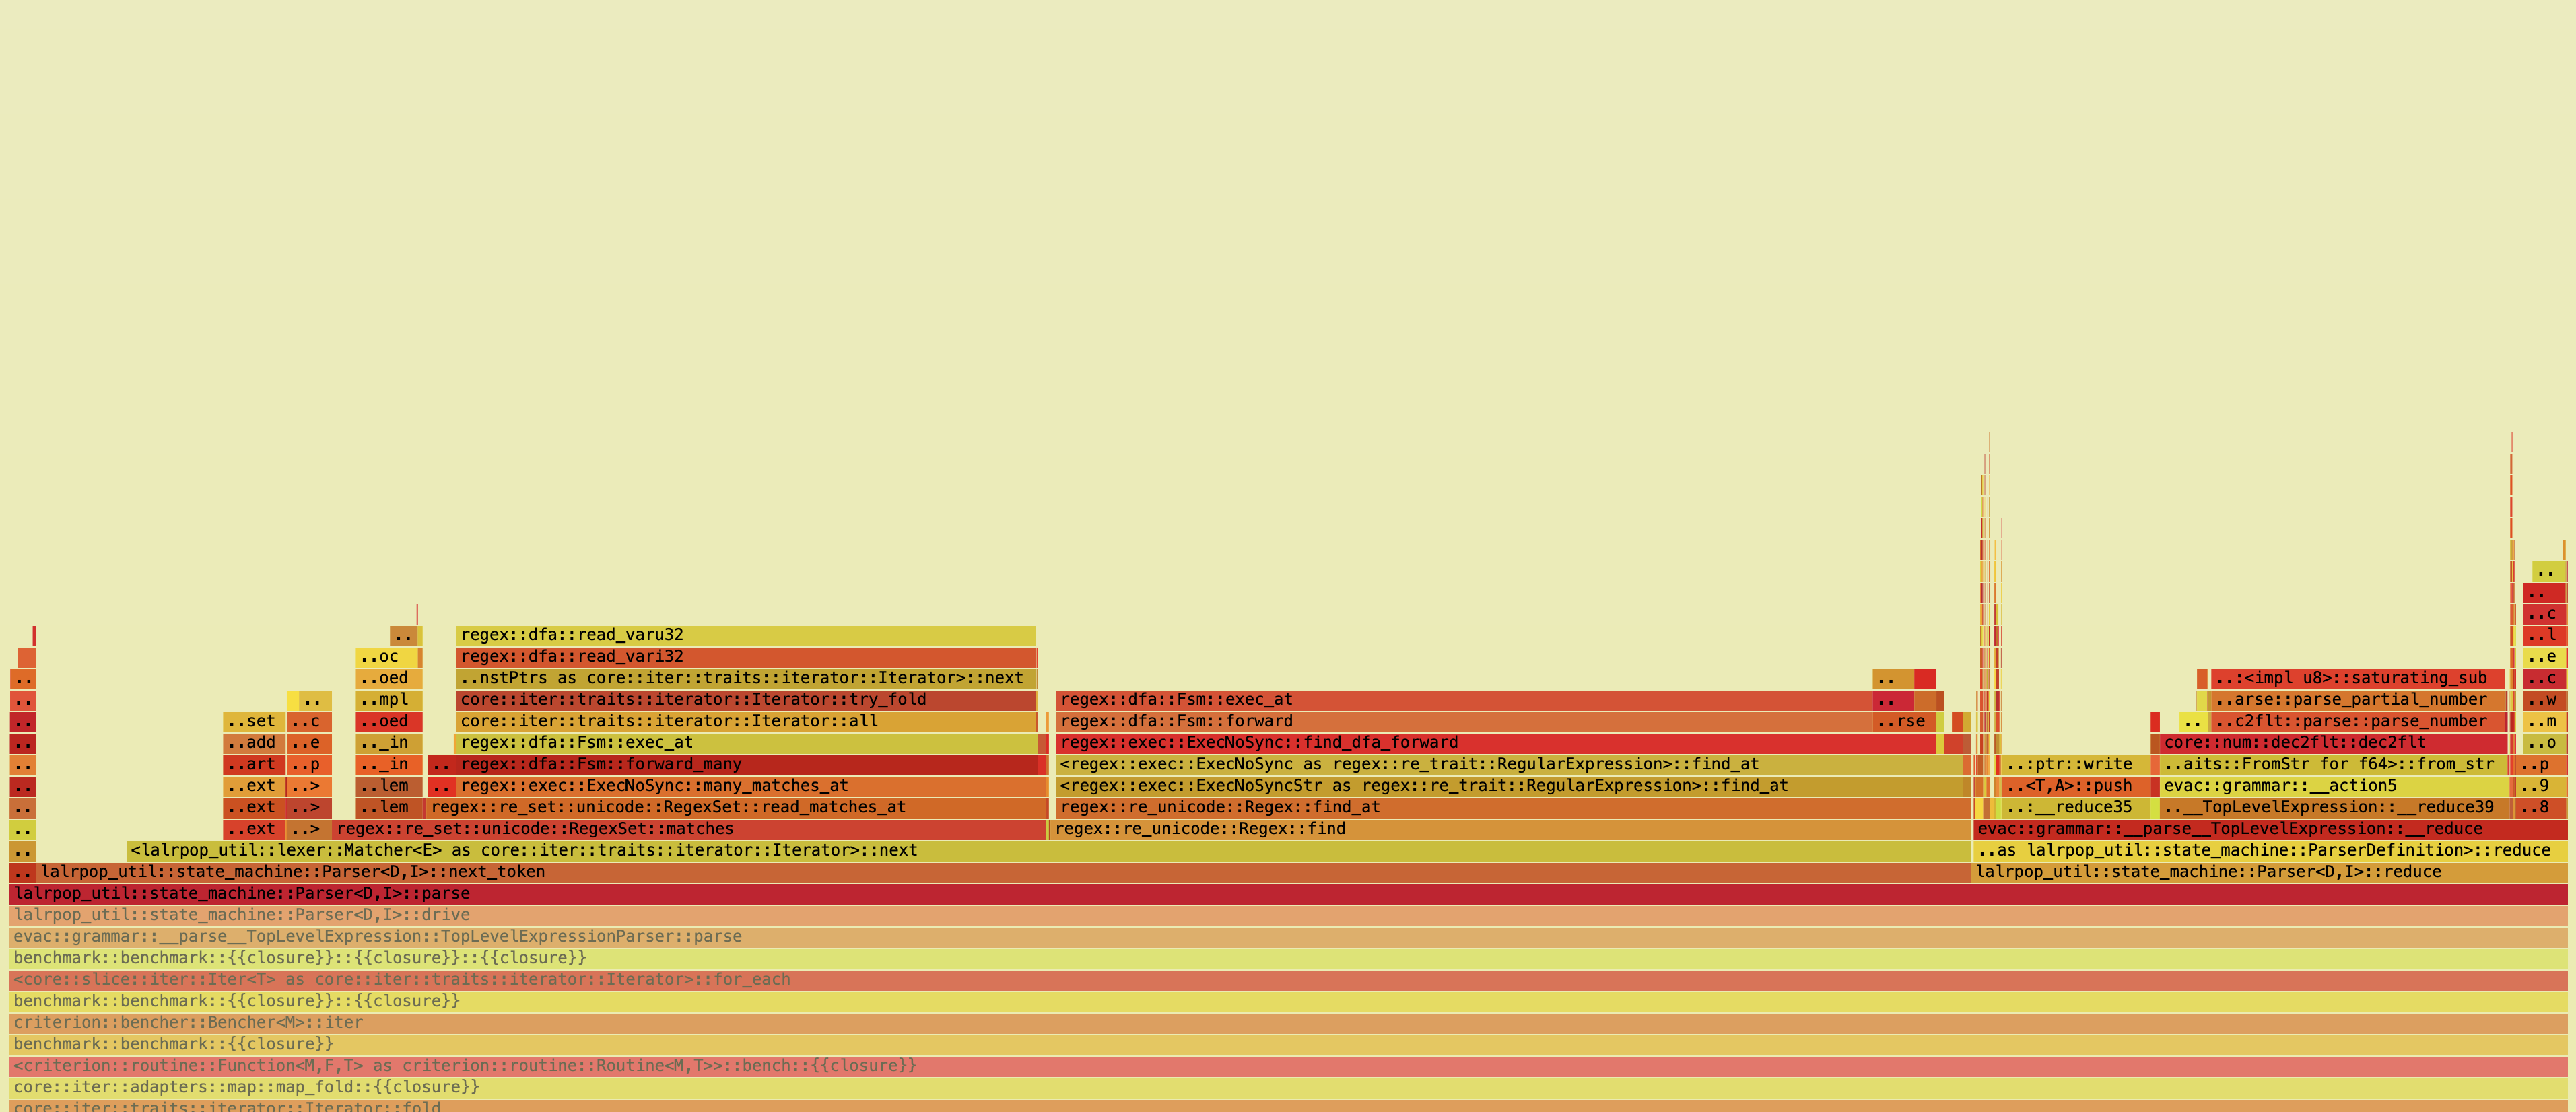
\includegraphics[width=\textwidth, height=0.8\textheight]{./fg_parse.png}
\end{frame}

\begin{frame}{Выводы}
  \begin{itemize}
    \item 70\% времени уходит на разбор следующего элемента лексером.
    \item 13\% времени уходит на разбор чисел с плавающей точкой
    \item Аллокации занимают 4\% времени, оптимизировать аллокатор не стоит.
    \item На текущих данных работа с hash-map не занимает много времени, но
          при экстремальных оптимизациях можно было бы использовать halfbrown.
  \end{itemize}
\end{frame}

\begin{frame}{Вычисление}
    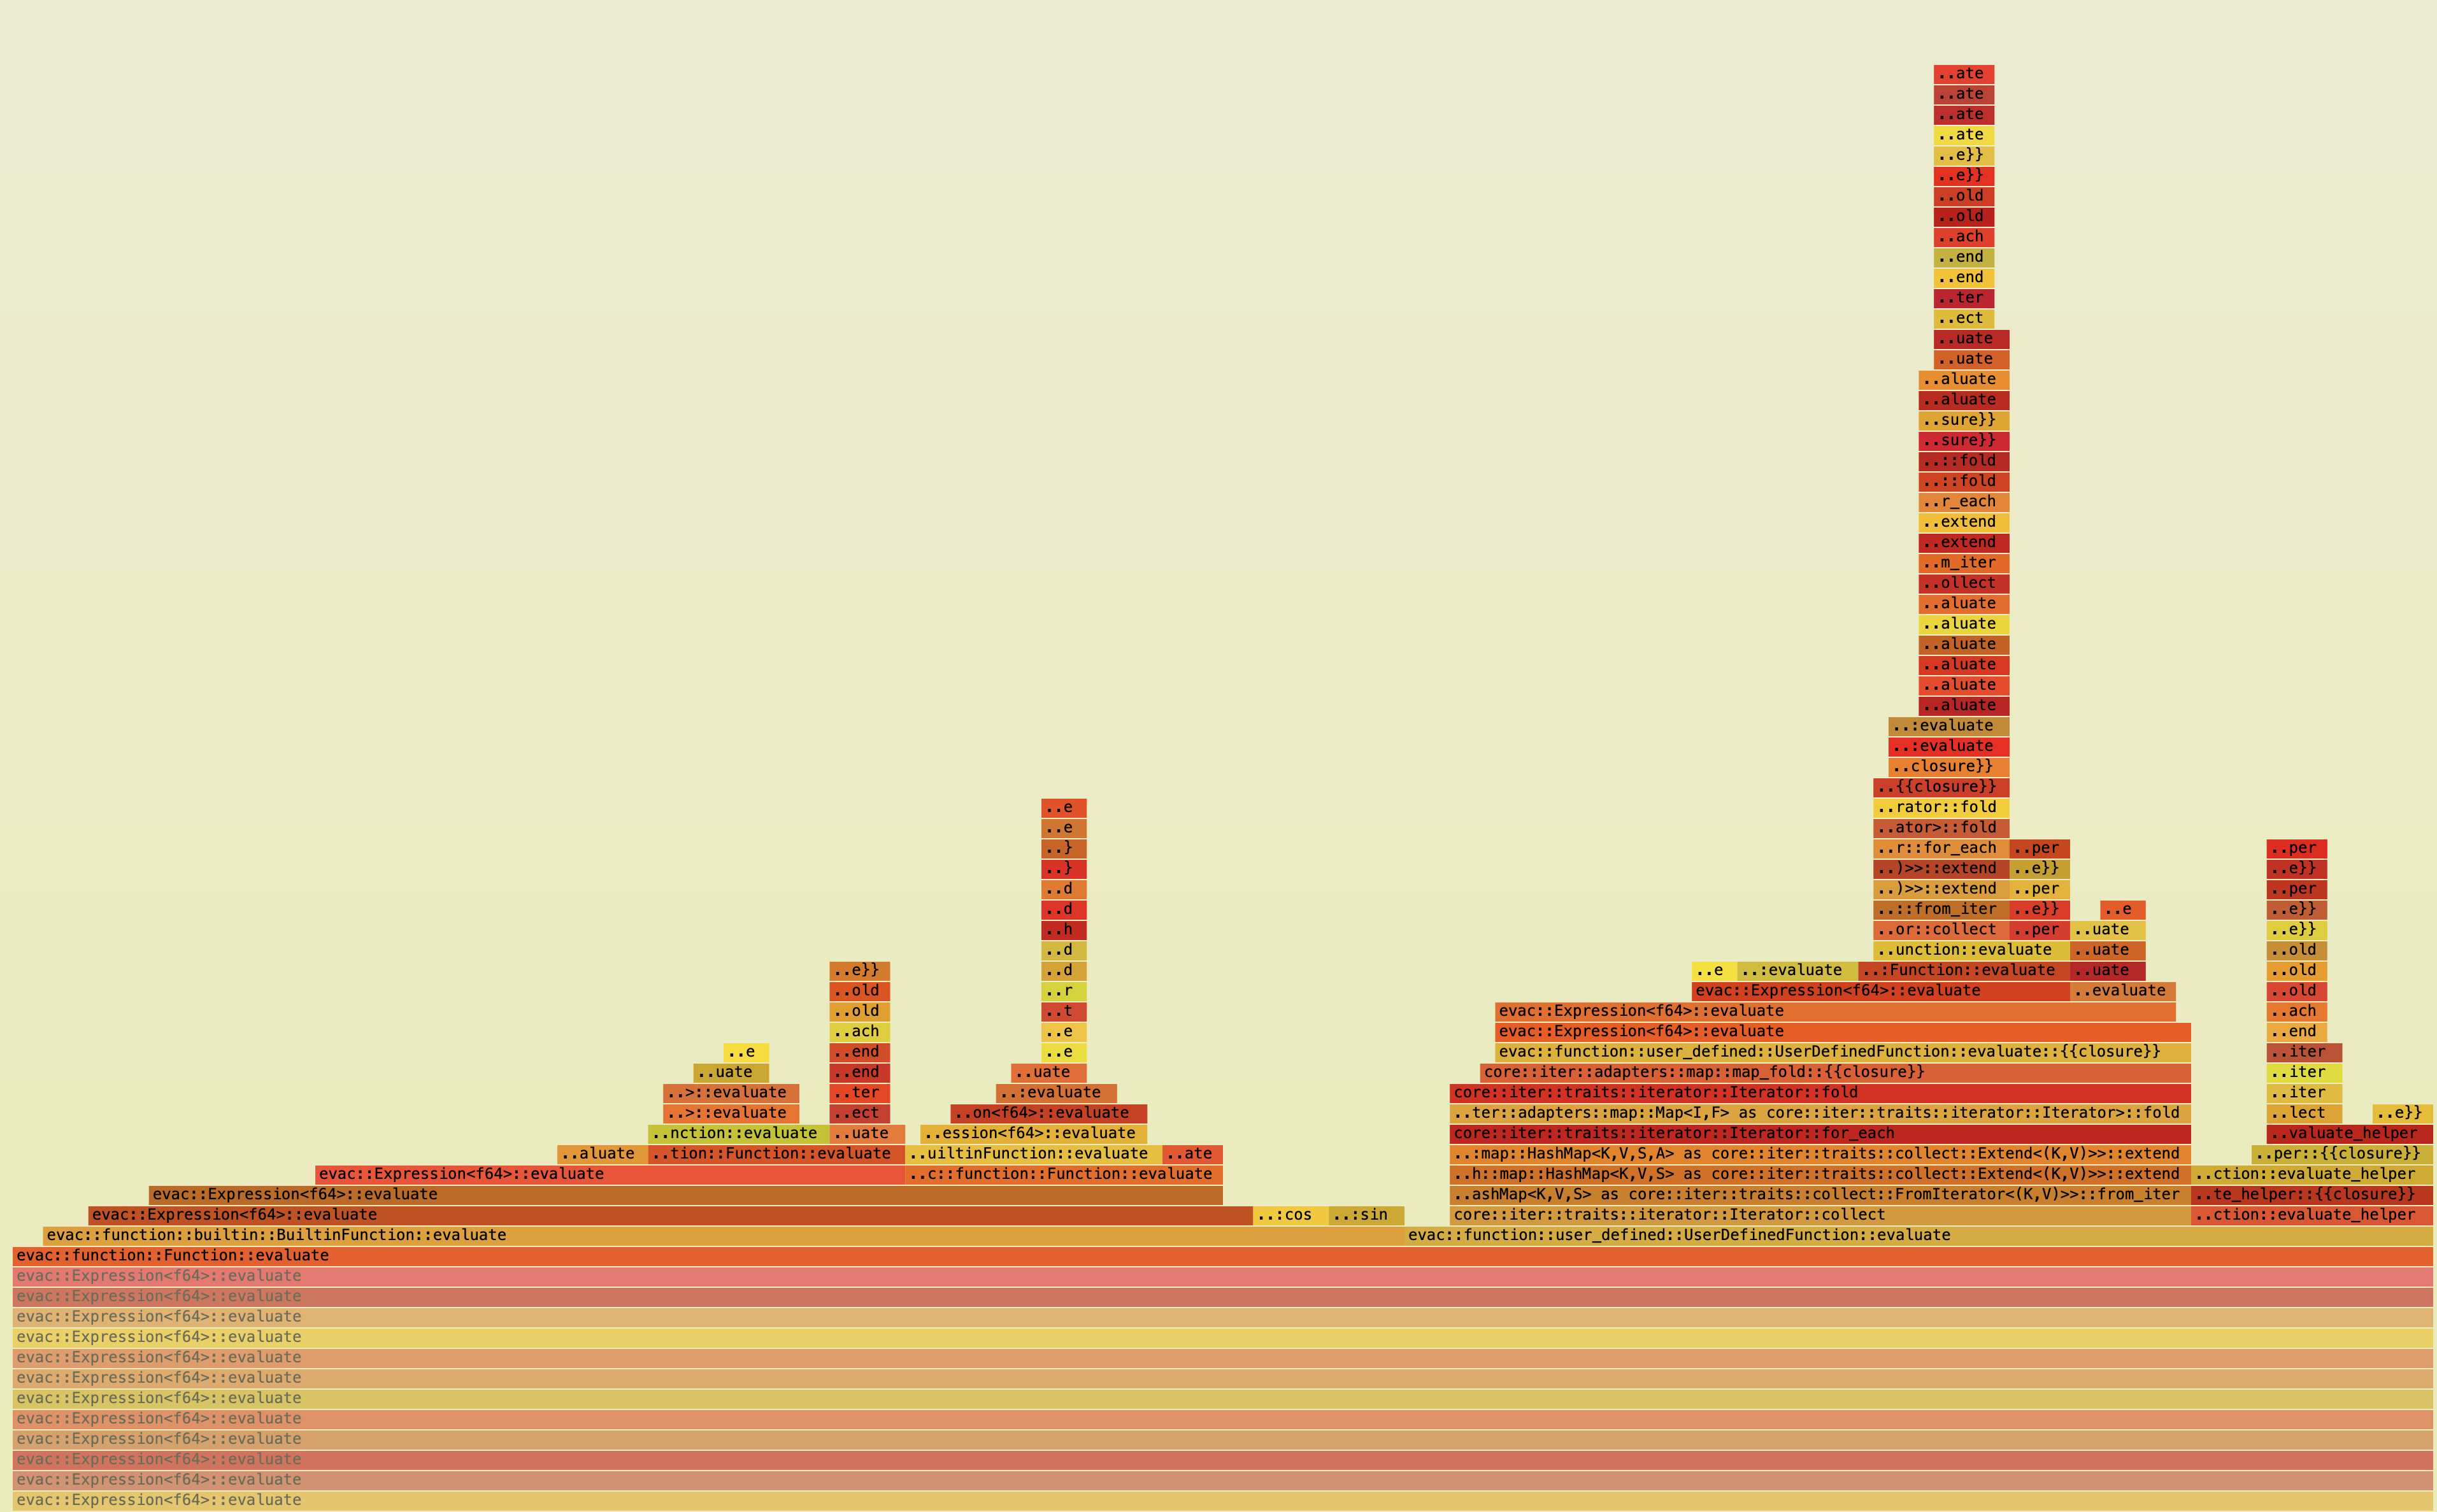
\includegraphics[width=\textwidth, height=0.8\textheight]{./fg_evaluate.png}
\end{frame}

\begin{frame}{Выводы}
  \begin{itemize}
    \item Профилировщик не умеет объединять срезы при рекурсивных вызовах.
    \item Интересующая нас часть находится в правой части и не сильно меняется
          между слоями.
  \end{itemize}
\end{frame}

\begin{frame}[fragile]
  \textbf{Локальность кэша}
\end{frame}

\begin{frame}
    \LARGE\begin{table}
        \begin{tabular}{|l|l|l|}
            \hline
                     & Такты & Размер       \\ \hline
            Регистры & 0     & несколько    \\ \hline
            L1       & 4     & 64КБ * ядро  \\ \hline
            L2       & 10    & 512КБ * ядро \\ \hline
            L3       & 50    & 64МБ         \\ \hline
            RAM      & 200   & 64ГБ         \\ \hline
        \end{tabular}
    \end{table}
\end{frame}

\begin{frame}{Задача:}
  \begin{itemize}
    \item Сделать наполнение одной кэш-линии максимально полным.
    \item Сделать расположение данных последовательным.
  \end{itemize}
\end{frame}

\begin{frame}[fragile]{Выражение}
    \begin{minted}[style = manni, fontsize=\small]{rust}
pub enum Expression<V> {
    Value(V),

    Op {
        left: Box<Self>,
        op: Operation,
        right: Box<Self>,
    },

    FnCall {
        function: Function,
        arguments: Vec<Self>,
    },
}
    \end{minted}
\end{frame}

\begin{frame}{Пути решения}
  \begin{itemize}
    \item Использовать арену (typed\_arena) или BUMP-аллокатор (bumpalo).
    \item Использовать SLAB-аллокатор (slab).
    \item Или.
  \end{itemize}
\end{frame}

\begin{frame}{Граф выражения}
    \begin{columns}[T,onlytextwidth]
        \begin{column}{0.5\textwidth}
            (1 * 2) + (3 / 4)
        \end{column}
        \begin{column}{0.5\textwidth}
            \usetikzlibrary {graphs, quotes}
            \tikz \graph [
               branch right = 2cm,
               grow down = 1.5cm,
               nodes={circle, draw}
            ] {
                "+" -> {
                    "*" -> { "1", "2" },
                    "/" -> { "3", "4" }
                }
            };
        \end{column}
    \end{columns}
\end{frame}

\begin{frame}[fragile]{Плоское представление}
\begin{table}[]
\begin{tabular}{|l|l|l|l|l|l|l|}
\hline
0          & 1          & 2   & 3   & 4          & 5   & 6   \\ \hline
op (+) 1 4 & op (*) 2 3 & v 1 & v 2 & op (/) 5 6 & v 3 & v 4 \\ \hline
\end{tabular}
\end{table}
\end{frame}

\begin{frame}[fragile]{Плоское вычисление}
\begin{table}[]
\begin{tabular}{|l|l|l|l|l|l|l|}
\hline
0          & 1          & 2   & 3   & 4          & 5   & 6   \\ \hline
op (+) 1 4 & op (*) 2 3 & v 1 & v 2 & op (/) 5 6 & v 3 & v 4 \\ \hline
2.75       & 2          & 1   & 2   & 0.75       & 3   & 4   \\ \hline
\end{tabular}
\end{table}
\end{frame}

\begin{frame}[fragile]
  \textbf{Оптимизация парсинга}
\end{frame}

\begin{frame}[fragile]
    \begin{minted}[style = manni, fontsize=\footnotesize]{rust}
#[derive(Debug, Clone, Copy, PartialEq, logos::Logos, derive_more::Display)]
pub enum Token<'input> {
    #[regex(r"-?\d+(\.\d*)?", float_parser)]
    Float(f64),

    #[regex(r"\p{alpha}+")]
    Name(&'input str),

    #[display(fmt = "fn")]
    #[token("fn")]
    Fn,

    ....

    #[error]
    #[regex(r"[ \t\n\f]+", logos::skip)]
    #[display(fmt = "")]
    Error,
}
    \end{minted}
\end{frame}

\begin{frame}[fragile]
    \begin{minted}[style = manni, fontsize=\large]{rust}
#[inline(always)]
fn float_parser<'input>(
    lex: &mut Lexer<'input, Token<'input>>
) -> f64 {
    fast_float::parse::<f64, &str>(lex.slice()).unwrap()
}
    \end{minted}
\end{frame}

\begin{frame}[fragile]
    \begin{minted}[style = manni, fontsize=\footnotesize]{rust}
extern {
    type Error = Error;
    type Location = usize;

    enum Token<'input> {
        "float" => Token::Float(<f64>),
        "+"     => Token::Sum,
        "-"     => Token::Sub,
        "*"     => Token::Mul,
        "/"     => Token::Div,
        "("     => Token::OpenBracket,
        ")"     => Token::CloseBracket,
        ","     => Token::Comma,
        "fn"    => Token::Fn,
        "="     => Token::Eq,
        ";"     => Token::Semicolon,
        "name"  => Token::Name(<&'input str>),
    }
}
    \end{minted}
\end{frame}

\begin{frame}[fragile]
    \begin{minted}[style = manni, fontsize=\scriptsize]{rust}
fn generate_names(count: usize) {
    let mut generator = regex_generate::Generator::new(
        r"\p{alpha}{2,12}",
        rand::thread_rng(), regex_generate::DEFAULT_MAX_REPEAT)
    .unwrap();

    let mut names = std::collections::HashSet::with_capacity(count);
    while names.len() < count {
        let mut buffer = vec![];
        generator.generate(&mut buffer).unwrap();
        let name = String::from_utf8(buffer).unwrap();
        names.insert(name);
    }

    let names: Vec<_> = names.into_iter().collect();
    let names = quote::quote! {
        pub(crate) const NAMES: [&str; #count] = [
            #(#names),*
        ];
    };

    std::fs::File::create("./src/names.rs")
        .unwrap()
        .write_all(names.to_string().as_bytes())
        .unwrap();
}
    \end{minted}
\end{frame}

\begin{frame}[fragile]
    Было:
    \begin{lstlisting}[basicstyle=\fontsize{10pt}{12}\bf\ttfamily\color{black}]
parse/3001              time:   [2.7657 s 2.7691 s 2.7722 s]
Found 10 outliers among 100 measurements (10.00%)
    \end{lstlisting}
    \hfill \break
    \hfill \break
    Стало:
    \begin{lstlisting}[basicstyle=\fontsize{10pt}{12}\bf\ttfamily\color{black}]
parse/3000              time:   [980.54 ms 981.29 ms 982.14 ms]
                        change: [-66.930% -66.863% -66.803%]
    \end{lstlisting}
\end{frame}

\begin{frame}[fragile]
  \textbf{Оптимизация вычисления}
\end{frame}

\begin{frame}[fragile]
    \begin{minted}[style = manni, fontsize=\footnotesize]{rust}
pub enum Layer<'input, V, N> {
    Value(V),

    Op {
        left: N,
        op: Operation,
        right: N,
    },

    FnCall {
        function: Function<'input>,
        arguments: Vec<N>,
    },
}
    \end{minted}
\end{frame}

\begin{frame}[fragile]
    \begin{minted}[style = manni, fontsize=\scriptsize]{rust}
impl<'input, A, B, V> MapLayer<B> for Layer<'input, V, A> {
    type To = Layer<'input, V, B>;
    type Unwrapped = A;

    #[inline(always)]
    fn map_layer<F: FnMut(Self::Unwrapped) -> B>(self, mut f: F) -> Self::To {
        match self {
            Layer::Value(v) => Self::To::Value(v),
            Layer::Op { left, op, right } => Self::To::Op {
                left: f(left),
                op,
                right: f(right),
            },
            Layer::FnCall {
                function,
                arguments,
            } => Self::To::FnCall {
                function,
                arguments: arguments.into_iter().map(f).collect(),
            },
        }
    }
}
    \end{minted}
\end{frame}

\begin{frame}[fragile]
    \begin{minted}[style = manni, fontsize=\small]{rust}
pub type TopBlockExpression<'input> = BlockExpression<'input, f64>;

pub struct BlockExpression<'input, V> {
    inner: RecursiveTree<Layer<'input, V, ArenaIndex>, ArenaIndex>,
}
    \end{minted}
\end{frame}

\begin{frame}[fragile]
    \begin{minted}[style = manni, fontsize=\scriptsize]{rust}
impl<'input, V: Copy> BlockExpression<'input, V> {
    #[inline]
    pub fn new(source: Expression<'input, V>) -> Self {
        Self {
            inner: RecursiveTree::expand_layers(source, |layer| match layer {
                Expression::Value(v) => Layer::Value(v),
                Expression::Op { left, op, right } => Layer::Op {
                    left: *left,
                    op,
                    right: *right,
                },
                Expression::FnCall {
                    function,
                    arguments,
                } => Layer::FnCall {
                    function,
                    arguments,
                },
            }),
        }
    }
}
    \end{minted}
\end{frame}

\begin{frame}[fragile]
    \begin{minted}[style = manni, fontsize=\footnotesize]{rust}
impl<'input> TopBlockExpression<'input> {
    pub fn evaluate(&self) -> f64 {
        self.inner.as_ref().collapse_layers(|node: Layer<f64, f64>| match node {
            Layer::Value(v) => v,
            Layer::Op { left, op, right } => op.evaluate(left, right),
            Layer::FnCall {
                function,
                arguments,
            } => function.evaluate(
                &arguments
                    .into_iter()
                    .map(Expression::Value)
                    .collect::<Vec<_>>(),
            ),
        })
    }
}
    \end{minted}
\end{frame}

\begin{frame}[fragile]
    \begin{minted}[style = manni, fontsize=\footnotesize]{rust}
proptest::proptest! {
    #[test]
    fn expression_equality(source in crate::properties::top_level_expression()
        .prop_filter("must be normal", |e| e.evaluate().is_normal()))
    {
        let evaluated = source.evaluate();

        let block = TopBlockExpression::new(source);
        prop_assert_eq!(evaluated, block.evaluate());
    }
}
    \end{minted}
\end{frame}

\begin{frame}[fragile]
    Было:
    \begin{lstlisting}[basicstyle=\fontsize{10pt}{12}\bf\ttfamily\color{black}]
not cache local/3000    time:   [79.177 ms 79.809 ms 80.617 ms]
Found 12 outliers among 100 measurements (12.00%)
    \end{lstlisting}
    \hfill \break
    \hfill \break
    Стало:
    \begin{lstlisting}[basicstyle=\fontsize{10pt}{12}\bf\ttfamily\color{black}]
cache local/3000        time:   [57.367 ms 57.671 ms 58.185 ms]
                        change: [-1.1773% -0.3219% +0.6466%]
    \end{lstlisting}
\end{frame}

\begin{frame}[fragile]
  \textbf{JIT-компиляция}
\end{frame}

\begin{frame}[fragile]
    \begin{minted}[style = manni, fontsize=\Large]{rust}
fn plus_two(foo) = foo + 2.0;
    \end{minted}
\end{frame}

\begin{frame}[fragile]
    \begin{minted}[style = manni, fontsize=\small]{rust}
// (1)
Expression::op(
  // (2)
  Expression::Value(
    // (3)
    FunctionValue::Variable("foo")
  ),
  // (6)
  Operation::Sum,
  // (4)
  Expression::Value(
    // (5)
    FunctionValue::Float(2.0)
  ),
)
    \end{minted}
\end{frame}

\begin{frame}[fragile]
    \begin{minted}[style = manni, fontsize=\large]{nasm}
.LCPI0_0:
        .quad   0x4000000000000000
plus_two:
        vaddsd  xmm0, xmm0, qword ptr [rip + .LCPI0_0]
        ret
    \end{minted}
\end{frame}

\begin{frame}{В экосистеме Rust}
  \begin{itemize}
    \item LLVM JIT: llvm-sys и inkwell
    \item Cranelift: cranelift
  \end{itemize}
\end{frame}

\begin{frame}{Джентельменский набор}
  \begin{itemize}
    \item Context - контекст LLVM JIT, в котором живёт всё остальное.
    \item Module  - модуль, в контексте которого мы будем определять функции.
    \item Builder - генератор LLVM IR для контекста.
    \item ExecutionEngine - контекст исполнения.
    \item PassManager - набор оптимизаций, который мы будем применять к функциям.
  \end{itemize}
\end{frame}

\begin{frame}[fragile]
    \begin{minted}[style = manni, fontsize=\fontsize{12}{12}]{rust}
pub struct Codegen<'ctx> {
    context: &'ctx Context,
    module: Module<'ctx>,
    builder: Builder<'ctx>,
    execution_engine: ExecutionEngine<'ctx>,
    pass_manager: PassManager<FunctionValue<'ctx>>,
}
    \end{minted}
\end{frame}

\begin{frame}[fragile]
    \begin{minted}[style = manni, fontsize=\scriptsize]{rust}
pub fn new(context: &'ctx Context) -> Self {
    let module = context.create_module("jit");
    let builder = context.create_builder();
    let execution_engine = module
        .create_jit_execution_engine(OptimizationLevel::Aggressive)
        .unwrap();

    let pass = PassManager::create(&module);
    pass.add_instruction_combining_pass();
    pass.add_instruction_simplify_pass();
    pass.add_new_gvn_pass();
    pass.add_cfg_simplification_pass();
    pass.add_reassociate_pass();
    pass.add_function_inlining_pass();
    pass.initialize();

    Self {
        context, module, builder,
        execution_engine,
        pass_manager: pass,
    }
}
    \end{minted}
\end{frame}

\begin{frame}[fragile]
    \begin{minted}[style = manni, fontsize=\footnotesize]{rust}
pub fn operation(
    &self,
    operation: Operation,
    left: FloatValue<'ctx>,
    right: FloatValue<'ctx>,
) -> FloatValue<'ctx> {
    match operation {
        Operation::Sum => self.builder.build_float_add(left, right, "sum"),
        Operation::Mul => self.builder.build_float_mul(left, right, "mul"),
        Operation::Div => self.builder.build_float_div(left, right, "div"),
        Operation::Sub => self.builder.build_float_sub(left, right, "sub"),
    }
}
    \end{minted}
\end{frame}

\begin{frame}[fragile]
    \begin{minted}[style = manni, fontsize=\scriptsize]{rust}
pub fn function_expression(&self, expression: &Expression<FValue>,
    function: &FunctionValue<'ctx>, args: &[&str],
) -> FloatValue<'ctx> {
    let expr = |expr| self.function_expression(expr, function, args);
    match expression {
        Expression::Value(FValue::Float(v)) => self.context.f64_type().const_float(*v),
        Expression::Value(FValue::Variable(v)) => {
            let index = args.iter().position(|a| a == v).unwrap();
            function.get_nth_param(index as u32).unwrap().into_float_value()
        }
        Expression::Op { left, op, right } => {
            let left = expr(left.as_ref());
            let right = expr(right.as_ref());
            self.operation(*op, left, right)
        }
        Expression::FnCall { function, arguments } => {
            let function = self.module.get_function(function.name()).unwrap();
            let args = arguments.iter().map(expr)
                .map(Into::<BasicMetadataValueEnum>::into)
                .collect::<Vec<_>>();
            self.builder.build_call(function, &args, "call")
                .try_as_basic_value().left().unwrap()
                .into_float_value()
        }
    }
}
    \end{minted}
\end{frame}

\begin{frame}[fragile]
    \begin{minted}[style = manni, fontsize=\footnotesize]{rust}
pub fn user_defined_function(
    &self,
    UserDefinedFunction { name, args, expression }: &UserDefinedFunction,
) -> FunctionValue {
    let f64_type = self.context.f64_type();
    let function_type = f64_type.fn_type(
        &vec![f64_type.into(); args.len()],
        false
    );
    let function = self.module.add_function(name, function_type, None);

    let basic_block = self.context.append_basic_block(function, "entry");
    self.builder.position_at_end(basic_block);

    let res = self.function_expression(expression, &function, args);
    self.builder.build_return(Some(&res));

    self.execution_engine.get_function_value(name).unwrap()
}
    \end{minted}
\end{frame}

\begin{frame}[fragile]
    \begin{minted}[style = manni, fontsize=\scriptsize]{rust}
let calls = (0..1000).map(|_| generate_correct_call()).collect_vec();

let jit_context = inkwell::context::Context::create();
let dataset = calls.clone().into_iter().map(|expr| {
    let codegen = Codegen::new(&jit_context);
    for f in  Context::from_expression(&expr).sort_calls() {
        codegen.user_defined_function(f.as_ref()).unwrap();
    }

    expr.jitify_inner(&codegen)
}).collect_vec();

c.bench_with_input(
    BenchmarkId::new("compiled calls", dataset_size),
    &dataset,
    |b, input| b.iter(|| input.iter().map(Expression::evaluate).sum::<f64>()),
);

c.bench_with_input(
    BenchmarkId::new("calls", dataset_size),
    &calls,
    |b, input| b.iter(|| input.iter().map(Expression::evaluate).sum::<f64>()),
);
    \end{minted}
\end{frame}

\begin{frame}[fragile]
    \begin{lstlisting}[basicstyle=\fontsize{10pt}{12}\bf\ttfamily\color{black}]
compiled calls/3000     time:   [495.00 µs 495.95 µs 496.93 µs]
Found 2 outliers among 100 measurements (2.00%)
  1 (1.00%) high mild
  1 (1.00%) high severe

calls/3000              time:   [666.45 µs 667.35 µs 668.36 µs]
Found 3 outliers among 100 measurements (3.00%)
  2 (2.00%) high mild
  1 (1.00%) high severe
    \end{lstlisting}
\end{frame}

\begin{frame}
  \textbf{В заключение}
\end{frame}

